\chapter{System Models}
\section{Scenarios}

The bindings do not affect core functionality of ROOT. Therefore 
we decided to give some examples on how the bindings might be used. The 
user in this case is a Node.js based application, that uses the rootJS bindings 
to interact with ROOT. As the actual implementation is not yet 
finalized, the scenarios only contain samples of simple interactions 
between an Application and ROOT.

\subsection{Web Viewer Scenario}
\begin{figure}[htb]
	\centering
	\begin{longtable}{p{3cm} @{\hskip 1cm} p{12cm}}
		\hline
		
		\textit{Scenario Name} & \underline{WebViewer}\\
		\hline
	
		\textit{Abstract} & A browser based GUI for realtime representation of root graphs.\\
		\hline
	
		\textit{Participating actor instances} & \underline{WebViewer:Node.js}; \underline{:ROOT}; \underline{:rootJS}\\
		\hline
	
		\textit{Flow of events} & 
		\begin{enumerate}
			\item rootJS is up and running initialize has already been executed.
			
			\item WebViewer calls the API method to get graphical output of the data ROOT has currently loaded.
				\begin{enumerate}
					\item rootJS processes the request and calls the corresponding ROOT functionality.
					\item rootJS receives ROOT output and streams it to WebViewer.
				\end{enumerate}
			\item WebViewer uses the provided data to display the graph on its GUI.
				\begin{enumerate}
					\item Node.js invokes ROOT I/O operations.
						\begin{enumerate}
							\item ROOT loads data and provides raw visualization data.
						\end{enumerate}
					\item Node.js serializes data and streams it to WebViewer.
				\end{enumerate}
			\item WebViewer receives data and renders it in the browser.
		\end{enumerate}
		\\
		\hline
		
	\end{longtable}
	
	\caption{WebViewer scenario}
	
\end{figure}

\pagebreak[4]

\subsection{Event Viewer Scenario}
\begin{figure}[htb]
	\centering
	\begin{longtable}{p{3cm} @{\hskip 1cm} p{12cm}}
		\hline
		\textit{Scenario Name} & \underline{EventViewer}\\
		\hline
		\textit{Abstract} &
		A Web based event viewer providing a visualisation of experimental data, showing signals particles have produced in the detector.
		The web viewer is split into the back-end, server part, with access to
	    the data source and enough resources to process the data, and the front-end, client part, that is a modern-enough Web browser, and responsible only for visualisation itself and interaction with the user.
		\\
		\hline
		\textit{Participating actor instances} & 
		\underline{Server:Node.js Application}; \underline{:ROOT}; \underline{EventViewer:Browser}; \underline{:rootJS}\\
		\hline
		\textit{Flow of events} &
		\begin{enumerate}
			\item EventViewer requests visual updates from Server.
			\item Server interfaces with ROOT via rootJS.
			\item ROOT acquires data from external source.
			\begin{enumerate}
					\item External, dedicated readout hardware is used to access the data source.
					\item ROOT processes incoming data in a timely manner.
			\end{enumerate}
			\item ROOT passes the data prepared for (3D) visualisation to the Server via rootJS.
			\item Server publishes its data as JSON stream over the web.
			\item EventViewer renders received data locally e.g. using WebGL.
		\end{enumerate}
		\\
		\hline
	\end{longtable}
	\caption{EventViewer scenario}
\end{figure}


\section{Use Cases}
Our bindings do not affect core functionality of ROOT. Therefore 
we decided to give some examples on how the bindings might be used. The 
user in this case is a nodeJS based application, that uses our bindings 
to interact with root. As the actual implementation is not yet 
finalized, our use cases only contain samples of simple interactions 
between an app and ROOT.
\begin{figure}[htb]
	\centering
	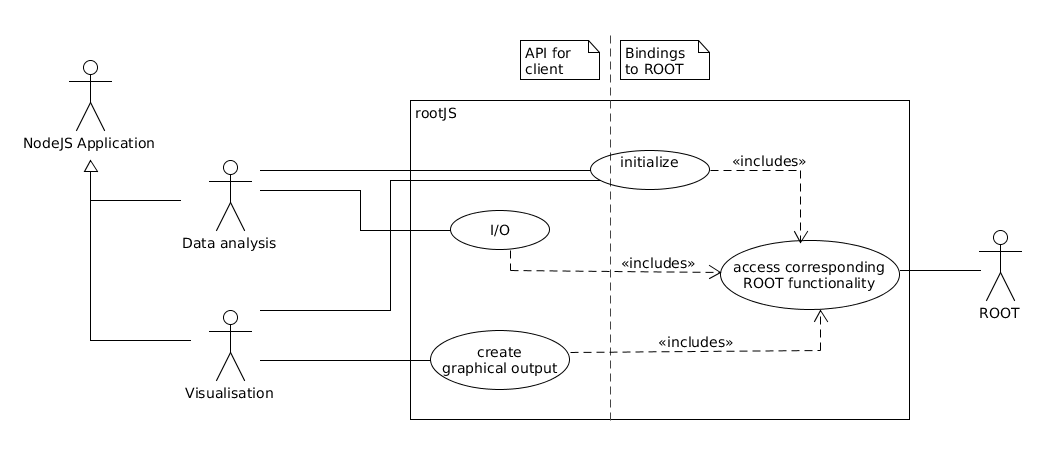
\includegraphics[width=18cm]{./latex/resources/usecaseOverview.png}
	\caption{use case overview}
\end{figure}

\pagebreak[4]

\subsection{Use Case 1: UseROOTConstant}

\begin{figure}[htb]
	\centering
	\begin{longtable}{p{3cm} @{\hskip 1cm} p{12cm}}
		\hline
		
		\textit{Use Case name} & \texttt{UseROOTConstant}\\
		\hline
		
		\textit{Participating actor instances} & Initiated by \texttt{NodeJSApplication}; Processed by \texttt{rootJS}; Communicates with \texttt{ROOT}\\
		\hline
		
		\textit{Flow of events} &
			\begin{enumerate}
				\item The \texttt{NodeJSApplication} requests access to a ROOT constant.
				\item \texttt{rootJS} sends a request to the corresponding ROOT constant.
				\item \texttt{ROOT} returns the requested value.
	                        \item The value is passed from \texttt{rootJS} to the \texttt{NodeJSApplication}.
			\end{enumerate}
			\\
		\hline
		
		\textit{Entry condition} & \texttt{rootJS} has been initialized\\
		\hline
		
		\textit{Exit condition} & The value has been returned to the NodeJSApplication\\
        \hline
	\end{longtable}
	
	\caption{Use Case: UseROOTConstant}
\end{figure}
\pagebreak
\subsection{Use Case 2: UseROOTClass}

\begin{figure}[htb]
	\centering
	\begin{longtable}{p{3cm} @{\hskip 1cm} p{12cm}}
		\hline
		
		\textit{Use Case name} & UseROOTClass\\
		\hline
		
		\textit{Participating actor instances} & Initiated by \texttt{NodeJSApplication}
                Processed by \texttt{rootJS}, ProxyObject
                Communicates with \texttt{ROOT}\\
		\hline
		
		\textit{Flow of events} &
			\begin{enumerate}
				\item The \texttt{NodeJSApplication}  requests access to a ROOT class by calling a constructor
				\item \texttt{rootJS} sends a request to the corresponding ROOT class
				\item \texttt{ROOT}  responds
				\item \texttt{rootJS} is allowed to create a ProxyObject of the requested
				ROOT class
				\item \texttt{rootJS} stores the ProxyObject in the cache
				\item \texttt{rootJS} returns the reference of the ProxyObject to the 
				\texttt{NodeJSApplication}
			\end{enumerate}
			\\
		\hline
		
		\textit{Entry condition} & \texttt{rootJS} has been initialized\\
		\hline
		
		\textit{Exit condition} & The reference of the ProxyObject has been return to the NodeJSApplication\\
        \hline
	\end{longtable}
	
	\caption{Use Case: UseROOTClass}
\end{figure}
\pagebreak
\subsection{Use Case 3: UseROOTFunction}

\begin{figure}[htb]
	\centering
	\begin{longtable}{p{3cm} @{\hskip 1cm} p{12cm}}
		\hline
		
		\textit{Use Case name} & UseROOTFunction\\
		\hline
		
		\textit{Participating actor instances} & Initiated by \texttt{NodeJSApplication}
                Processed by \texttt{rootJS}, ProxyObject
                Communicates with \texttt{ROOT}\\
		\hline
		
		\textit{Flow of events} &
			\begin{enumerate}
				\item The \texttt{NodeJSApplication}  requests access to a ROOT function
				\item \texttt{rootJS} sends a request to the corresponding ROOT function
				\item \texttt{ROOT}  responds
				\item \texttt{rootJS} is allowed to create a ProxyObject of the class where the requested ROOT function is located
				\item The ProxyObject calls the requested ROOT function
				\item \texttt{rootJS} returns the output of the function ProxyObject to the 
				\texttt{NodeJSApplication}
			\end{enumerate}
			\\
		\hline
		
		\textit{Entry condition} & \texttt{rootJS} has been initialized\\
		\hline
		
		\textit{Exit condition} & The reference of the ProxyObject has been return to the NodeJSApplication\\
        \hline
	\end{longtable}
	
	\caption{Use Case: UseROOTFunction}
\end{figure}



\pagebreak[4]

\section{Object Models}
Figure 6.2 illustrates what the rootJS architecture may look like.
Client applications relying on this architecture will incorporate with the ROOT framework through a \textit{ROOTPrototype} object.
The API's entry point method \textit{ROOTPrototype::init} uses V8 to create the actual interface to the available variables, functions and classes of ROOT.\\
Functions provided through this interface internally call \textit{methodProxy} to determine the associated ROOT function via the callee's function name. This allows handling of supplied callback functions by passing them over the \textit{args} parameter.\\
Constructor functions provided through the interface internally call \textit{classProxy} instead of \textit{methodProxy} to generate encapsulating JavaScript objects through the \textit{ProxyObjectFactory}.
A \textit{ROOTPrototype} object provides the \textit{globalGetter} and \textit{globalSetter} methods to access ROOT's global variables. Again interfacing with global objects is done through \textit{ProxyObject}s generated by the \textit{ProxyObjectFactory}.
\\ \\
The \textit{ProxyObjectFactory} instantiates a class realizing the \textit{ProxyObject} interface. The actual class type is given through the supplied \textit{type} parameter.
If the \textit{getV8Handle} method is called on \textit{ProxyObject}s encapsulating C++ scalar types (like int, long, string, etc.) it will simply return the corresponding \textit{v8::Handle} with the value at a defined address in memory.\\
However, calling the \textit{getV8Handle} method on \textit{ProxyObject}s encapsulating C++ objects will prompt recursive calls to the \textit{ProxyObjectFactory} for every (member) variable the native object holds. This allows to dynamically assemble the encapsulating object.
To handle cyclic references a caching mechanism (\textit{ProxyObjectCache}), that stores already created \textit{v8::Handle}s, is used.\\
A sample process of interfacing with a ROOT object using this architecture is shown in Figure 6.4.

\begin{figure}[htb]
	\centering
	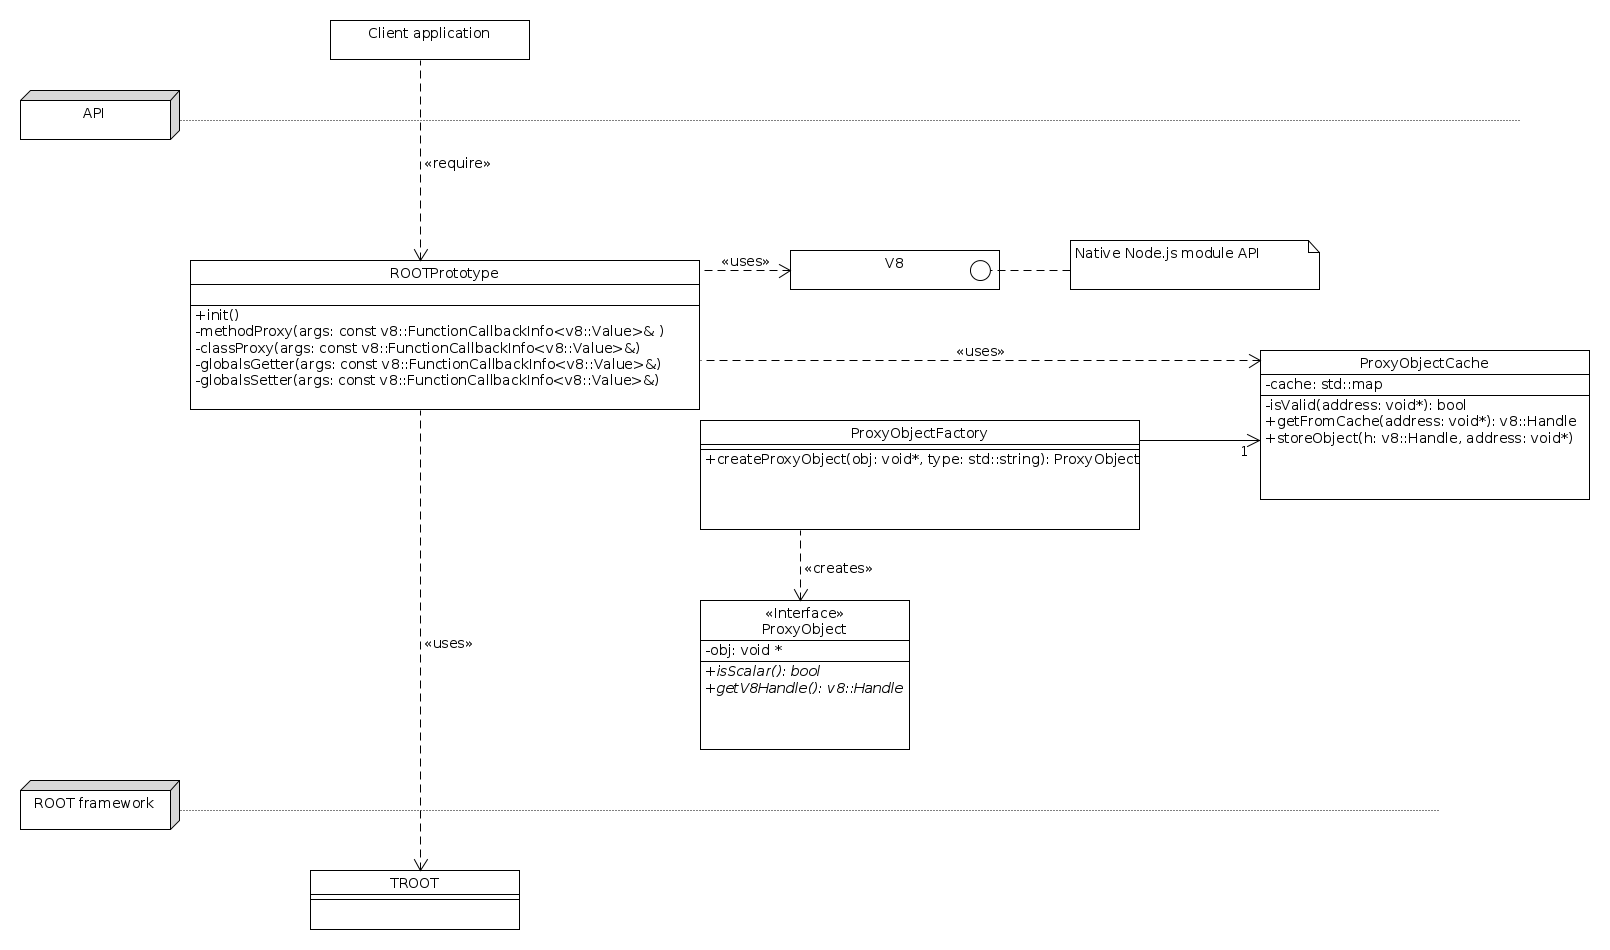
\includegraphics[width=18cm]{./latex/resources/architecture.png}
	\caption{basic architecture draft}
\end{figure}

\pagebreak[4]

\section{Dynamic Models}
The following figure shows how rootJS initializes upon being called the first time by a client application. As bindings do not add any functionality of their own, the client application is not further specified. After the bindings are initialized the client application may use any ROOT functionality through a \textit{ROOTPrototype} object provided by the rootJS API.

\begin{figure}[htb]
	\centering
	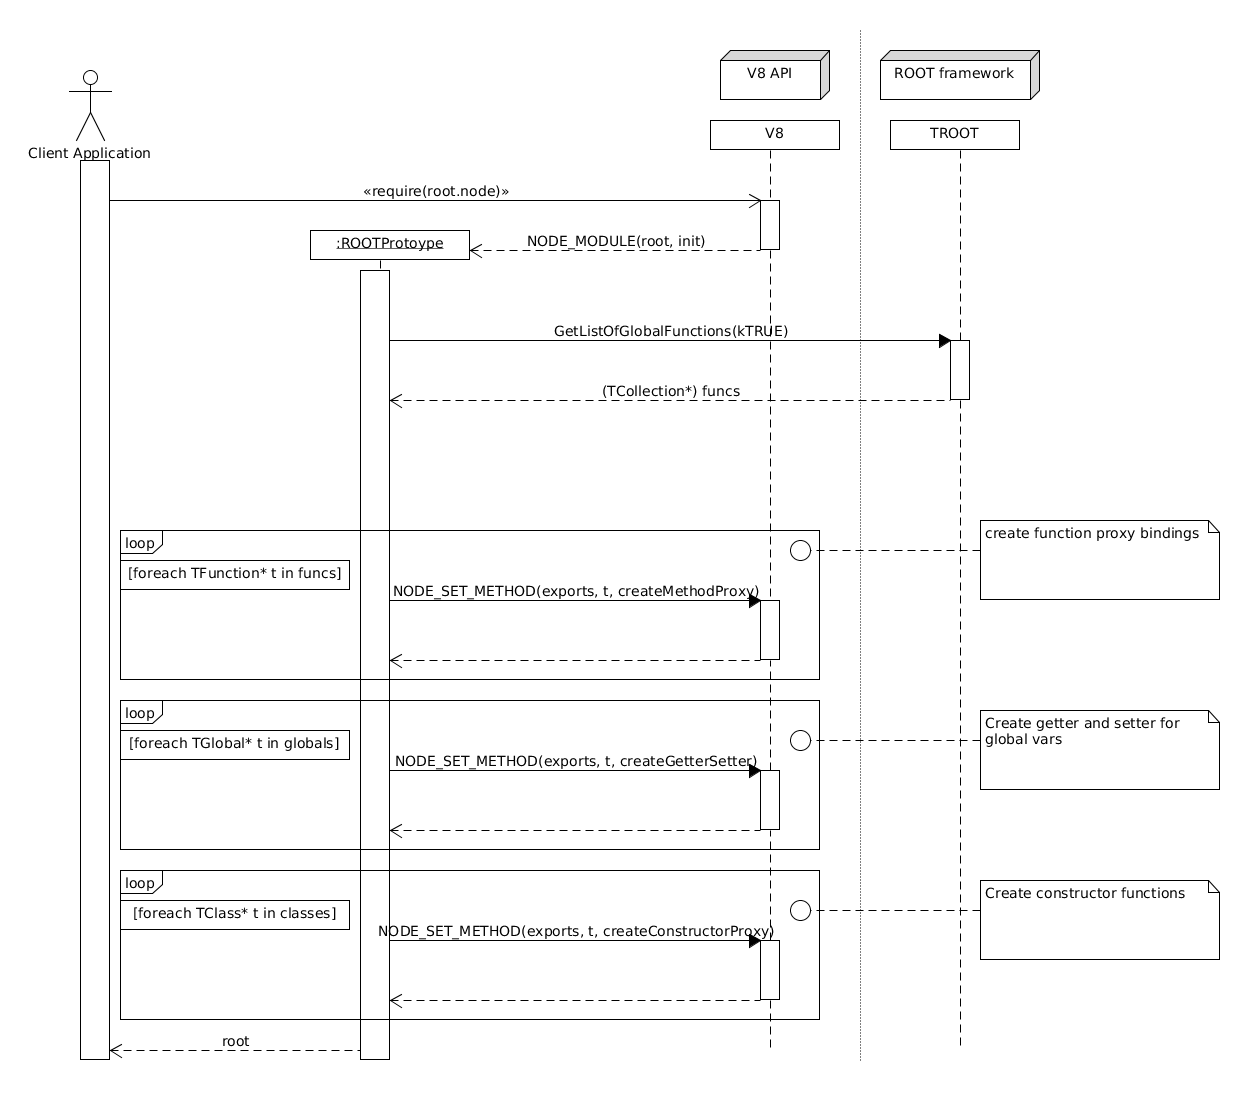
\includegraphics[width=18cm]{./latex/resources/startupSequence.png}
	\caption{basic startup sequence}
\end{figure}

The following figure shoes how to open a root file via rootJS, after the usual initialization process has been completet (see above) a TFile object is beeing created using the rootJS API. A callback is provided because the file is beeing parsed by ROOT during the opening process, which might take some time depending on file size and complexity. The rootJS bindings call the TFile constructor before returning to the JavaScript application via callback, the constructor is beeing called by the class proxy. After the construction phase rootJS has a valid TFile object, which is then handed over to the CreateProxyObject factory method which creates the correct proxy object. The factory object recursively creates a v8 handle which is returned to the JavaScript code running in node, in this case via callback.
\begin{figure}[htb]
	\centering
	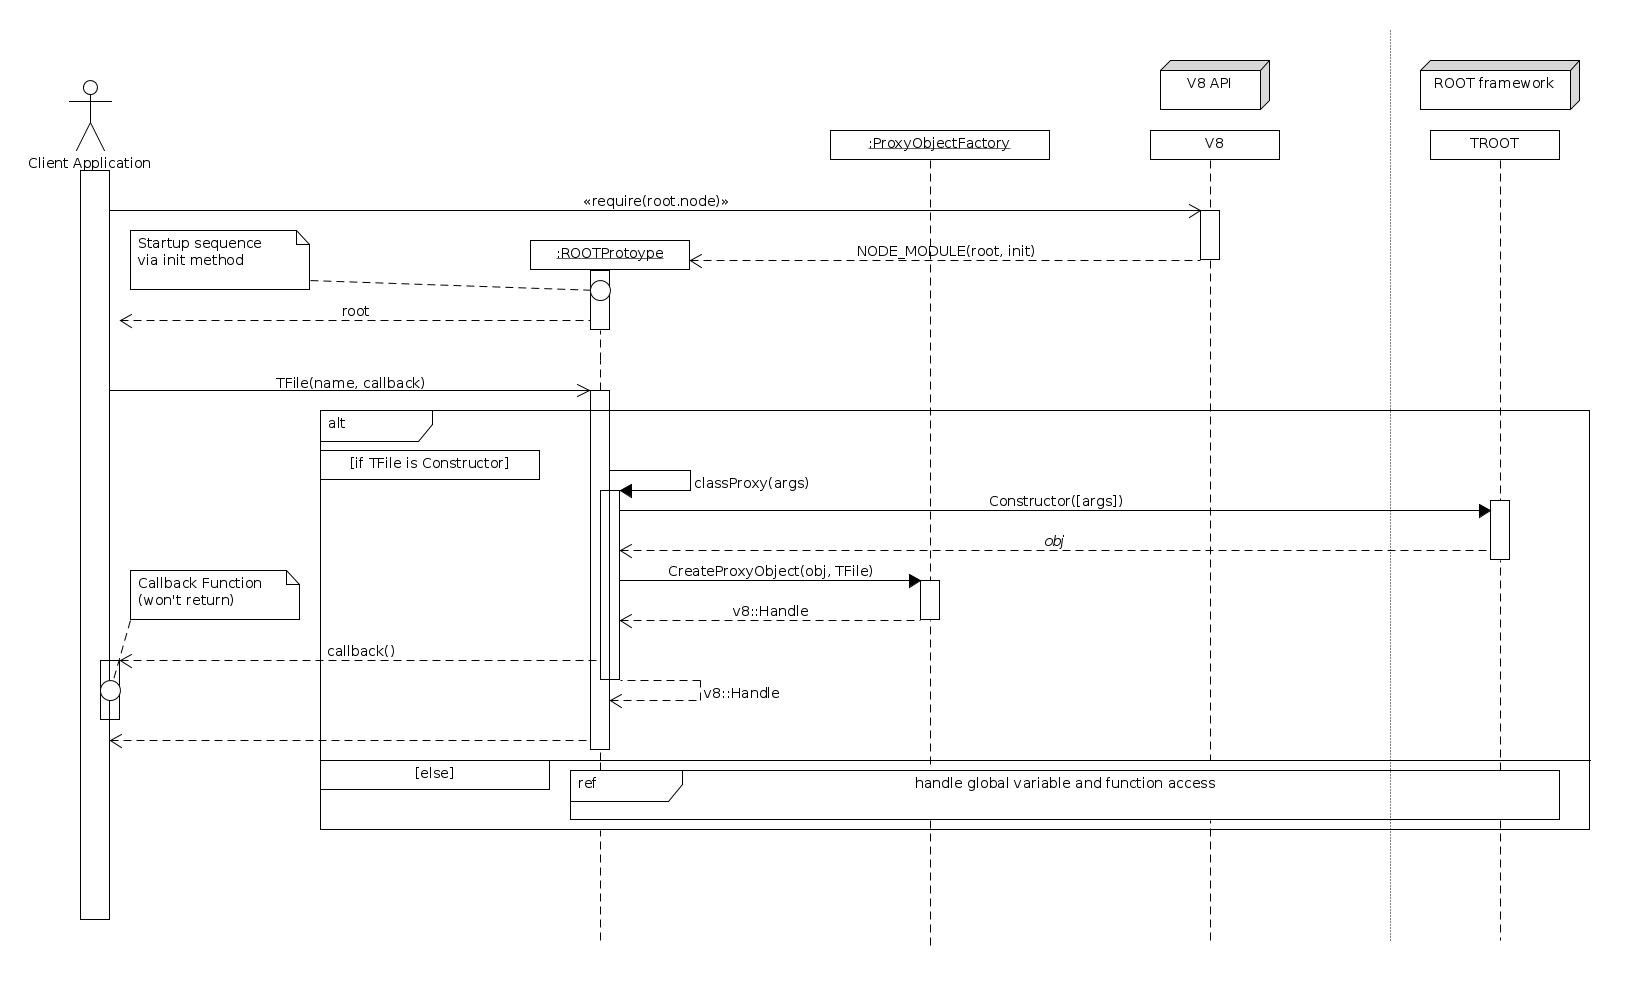
\includegraphics[width=18cm]{./latex/resources/fileOpen.png}
	\caption{basic sequence used for opening a file}
\end{figure}
